\section{Spielbeschreibung}

\begin{figure}[hbt]
  \centering
  
\includegraphics[width=0.45\textwidth,angle=0]{graphics/ligretto.jpg}
  \caption{Ligretto \hfill{} }
 \end{figure}

Ligretto ist ein Spiel, bei dem es darum geht, seinen eigenen Ligretto Stapel los zu werden bevor dies ein Gegner schafft. Der Ligretto Stapel besteht aus 10 verdeckten zufälligen Karten aus dem Kartenvorrat des Spielers. Der Kartenvorrat eines Spielers (auch Deck genannt), besteht aus 40 Karten. Die Karten sind von 1 bis 10 nummeriert und haben die folgenden vier Farben: Rot, Gelb, Blau und Grün. Es gibt keine doppelten Karten, das heisst, jede Karte kommt nur genau einmal im Deck des Spielers vor.

\begin{figure}[hbt]
  \centering
  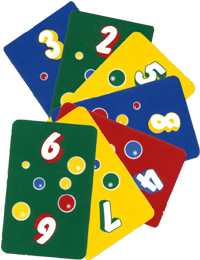
\includegraphics[width=0.20\textwidth,angle=0]{graphics/ligretto.png}
  \caption{Ligretto Karten \hfill{} }
 \end{figure}

Um ein neues Spiel vorzubereiten, mischt jeder Spieler seinen Kartenstapel. Jeder Spieler zählt dann 10 Karten ab und legt diese verdeckt vor sich hin. Dies ist sein eigener Ligretto Stapel. Danach legt er 4 Karten von seinen restlichen Handkarten offen neben den Stapel. Sobald alle Spieler soweit sind, geht es los.

Der Spielablauf funktioniert nun für jeden Spieler wie folgt. Der Spieler
\begin{enumerate}
\item schaut die offen vor sich liegenden Karten an,
\item prüft die Stapel an Karten in der Mitte des Spielfelds und
\item versucht nun eine Karte zu finden, die eins höher ist als die oberste Karte eines Stapels und die selbe Farbe besitzt. Ist dies der Fall, so darf er seine Karte nehmen und oben auf diesen Stapel legen.
\item Wenn diese gelegte Karte eine der vier offen vor sich liegenden Karten gewesen ist, dann darf der Spieler die oberste Karte vom Ligretto Stapel aufdecken und anstelle der soeben gelegten Karte vor sich hin legen.
\item Wenn eine 1er Karte verfügbar ist, darf damit ein neuer Stapel in der Mite des Spielfelds eröffnet werden.
\item Wenn mit den offenen Karten keine Aktionen durchgeführt werden können darf der Spieler von seinen restlichen Handkarten 3 Karten verdeckt abzählen und diese umdrehen und vor sich auf den Ablagestapel legen. Existiert noch kein Ablagestapel so legt er die 3 Karten neben seine bereits vor sich liegenden Karten und eröffnet somit seinen Ablagestapel. Beim Ablagestapel darf nun jeweils die oberste Karte ebenfalls gespielt werden.
\item Sollte weiterhin keine Karte gelegt werden können, so wiederholt der Spieler Punkt 6 und legt immer 3 Karten oben auf den Ablagestapel, bis er keine Handkarten mehr in der Hand hält. Ist dies der Fall, so nimmt der Spieler den Ablagestapel wieder als Handkarten auf und fängt von vorne an.
\end{enumerate}

Sobald ein Spieler die letzte Karte seines Ligretto Stapels aufgedeckt hat, ruft er \textit{Ligretto Stop!}, das Spiel wird beendet und es wird abgerechnet.

Bei der Abrechnung bekommt jeder Spieler Punkte für sich selber. Die Abrechnung läuft wie folgt ab:
\begin{enumerate}
	\item Jeder Spieler zählt die noch vorhandenen Karten auf dem eigenen Ligretto Stapel. Für jede Karte auf dem Ligretto Stapel bekommt er zwei Minuspunkte.
	\item Die Karten auf dem Spielfeld werden nun wieder nach Farbe auf der Rückseite sortiert. Jeder Spieler erhält seine Karten zurück und zählt diese. Für jede gelegte Karte bekommt der Spieler einen Pluspunkt.
	\item Die Punkte werden nun notiert und  jeder Spieler bereitet sich für die nächste Runde vor.
\end{enumerate}